\documentclass[a4paper, 11pt]{article}
\usepackage[english]{babel}
\usepackage[utf8]{inputenc}
\usepackage{amsmath}
\usepackage{graphicx}
\usepackage{float}
\usepackage{fixltx2e}
\usepackage{listings}
\usepackage{color}
\usepackage{latexsym}
\usepackage{lstautogobble}
\usepackage[colorinlistoftodos]{todonotes}
\usepackage[margin=3cm]{geometry}
\usepackage{hyperref}
\usepackage{libertine}
\usepackage{tikz}
\hypersetup{
	hidelinks, 
	colorlinks = true,
	linkcolor = black,
}

\usetikzlibrary{shapes, arrows}

\newtheorem{definit}{Definizione}[subsection]

\begin{document}
	\clearpage
	\begin{titlepage}
		\centering
		\vspace*{\fill}
		{\scshape\LARGE Università degli Studi di Verona \par}
		\vspace{1.5cm}
		\line(1,0){230} \\
		{\huge\bfseries Sicurezza delle reti\par}
		\line(1,0){230} \\
		\vspace{0.5cm}
		{\scshape\Large Riassunto dei principali argomenti\par}
		\vspace{2cm}
		{\Large\itshape Davide Bianchi\par}
		\vspace{1cm}
		\vspace{5cm}
		\vspace*{\fill}
		% Bottom of the page
		{\large \today\par}
	\end{titlepage}
	\thispagestyle{empty}
	\newpage
	\tableofcontents
	\newpage
	
	\section{Introduzione}
	
	\begin{definit}[Information Security]
		Protezione delle informazioni e dei sistemi per impedirne l'accesso non autorizzato, uso, divulgazione, modifica o distruzione.
	\end{definit}
	
	\begin{definit}[Network Security]
		Protezione dell'accesso a risorse situate all'interno di una rete.
	\end{definit}
	
	Nella sicurezza si distinguono una \textbf{policy}, un \textbf{meccanismo} e una \textbf{compliance}.
	Una security policy specifica il comportamento che il sistema può o non può assumere. I meccanismi di sicurezza sono l'implementazione di una data policy. Diciamo quindi che una security policy $\phi$ deve rimanere valida per un sistema $P$ in ogni ambiente malevolo $E$, ovvero $P \parallel E \models \phi $.
	
	Le politiche di sicurezza sono spesso formulate per arrivare ad alcune proprietà standard, le più comuni sono:\begin{itemize}
		\item Confidenzialità: non ci sono fughe di informazioni;
		\item Integrità: non ci sono modifiche alle informazioni;
		\item Disponibilità: non ci sono "danneggiamenti" ai servizi;
		\item Accountability\footnote{La traduzione più vicina è \textit{responsabilità}.}: le azioni sono sempre riconducibili ai diretti responsabili;
		\item Autenticazione: l'origine dei dati può essere identificata con sicurezza.
	\end{itemize}
	
	\paragraph{Contromisure per la protezione.} Le principali tecniche di contromisura consistono in:\begin{itemize}
		\item Prevenzione di breach;
		\item Rilevamento di attacchi in corso;
		\item Reazione ad un possibile attacco.
		\end{itemize}
		
	\section{Cenni di crittografia}
	\subsection{Introduzione}
	Iniziamo dando alcune definizioni fondamentali. Si useranno i termini \textit{ciphertext} e \textit{plaintext} per indicare rispettivamente il testo cifrato e quello in chiaro.
	
	\begin{definit}[Crittografia]
	Insieme dei metodi per rendere un messaggio non leggibile ad altri.
	\end{definit}
	
	\begin{definit}[Steganografia]
	Insieme dei metodi per nascondere l'esistenza di un messaggio in un altro contenuto.
	\end{definit}
	
	\begin{definit}[Crittoanalisi]
	Analisi del ciphertext per ottenere il plaintext corrispondente.
	\end{definit}
					
	Un generico sistema crittografico è strutturato come: \\
	
	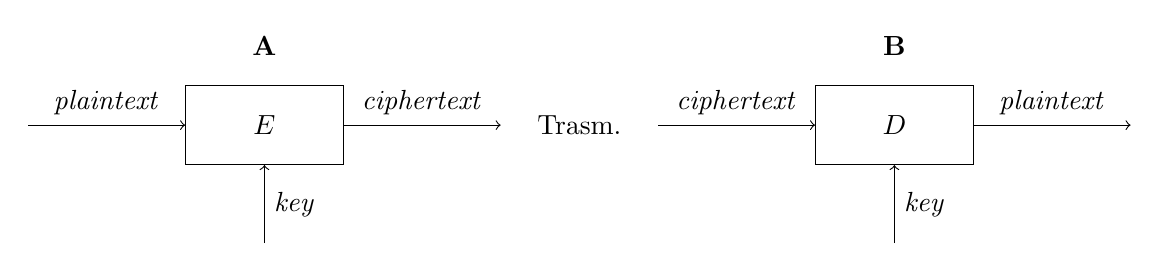
\begin{tikzpicture}
	\node at (4,0) [rectangle,draw, minimum width=2cm, minimum height=1cm] (E) {$E$};
	\draw (E);
	\draw[->] (1,0) -- (E) node[above, midway] {\textit{plaintext}};
	\draw[->] (4,-1.5) -- (E) node[right, midway] {\textit{key}};
	\draw[->] (E) -- (7,0) node[above, midway] {\textit{ciphertext}};
	\node at (8,0) (dots) {Trasm.};
	\node at (12,0) [rectangle,draw, minimum width=2cm, minimum height=1cm] (D) {$D$};
	\draw[->] (9,0) -- (D) node[above, midway] {\textit{ciphertext}};
	\draw[->] (12,-1.5) -- (D) node[right, midway] {\textit{key}};
	\draw[->] (D) -- (15,0) node[above, midway] {\textit{plaintext}};
	\node at (4,1) {\textbf{A}};
	\node at (12,1) {\textbf{B}};
	\end{tikzpicture}
	
	In crittografia si distinguono le due categorie \textit{a chiave simmetrica} e \textit{a chiave asimmetrica}. La differenza sta nel fatto che nella crittografia a chiave simmetrica le due entità che si scambiano il messaggio devono condividere una stessa chiave (che deve essere trasmessa su un canale sicuro), mentre nella crittografia a chiave asimmetrica le chiavi sono differenti e sono 2 per ogni entità, una pubblica e una privata. Nella crittografia a chiave asimmetrica si elimina il problema della condivisione della chiave; inoltre la chiave pubblica può essere compromessa da attaccanti senza che la chiave privata venga compromessa, e senza che venga compromessa la segretezza del messaggio.
	
	Un altro aspetto fondamentale della crittografia è che la cifratura e la decodifica sono facili, \textit{se le chiavi sono note}. Da ciò consegue che la sicurezza debba risiedere nella chiave, non nell'algoritmo in se.
	
	\subsection{Crittoanalisi}
	La scienza di recuperare il messaggio in chiaro senza conoscere il ciphertext si basa sostanzialmente su due differenti approcci:
	\begin{itemize}
		\item attacco brute-force;
		\item attacco crittoanalitico.
	\end{itemize}
	
	\paragraph{Attacco brute-force.} Un attacco bruteforce è semplice: consiste nel provare tutte le chavi possibili fino ad indovinare quella corretta. Questa tipologia di attacco in generale è sempre possibile nella sua semplicità, tuttavia, se la dimensione dello spazio delle chiavi inizia ad essere elevata, il tempo che si deve impiegare diventa insostenibile, per cui in questi casi è necessario ricorrere ad altri stratagemmi.
	
	\paragraph{Attacco crittoanalitico.} In questo caso si assume che l'attaccante conosca l'algoritmo utilizzato nella cifratura dei messaggi; si trova quindi una qualche debolezza nell'algoritmo che permetta di farlo fallire. 
	
	In tal senso, si tende a rendere noto un algoritmo affinchè il maggior numero di persone tenti di attaccarlo, per aumentare al massimo le possibilità che venga trovata una falla. (In contrasto con la cosiddetta \textbf{security by obscurity}).
	
	\paragraph{Tipologie di attacco.}Consideriamo ora i possibili attacchi che un sistema crittografico deve affrontare per essere affidabile:
	\begin{itemize}
		\item \textit{known cypertext attack:} questo attaccante è il meno aggressivo e conosce solamente il testo cifrato;
		
		\item \textit{known plaintext attack:} conosce entrambi i tipi di testo;
		
		\item \textit{choosen plaintext:} può scegliere il plaintext da codificare e analizzare il ciphertext ottenuto;
		
		\item \textit{adaptive choosen plaintext:} può liberamente scegliere il plaintext da far codificare e comportarsi di conseguenza, sulla base del risultato appena ottenuto.
		
		\item \textit{chosen ciphertext:}l'attaccante può scegliere differenti ciphertext e avere accesso al plaintext decriptato, per infine ricavare la chiave.
		\end{itemize}
	
	
	
	
	
	
	
	
	
	
	
	
	
	
	
	
	

\end{document}